\subsection {Técnicas de agrupamiento (Clustering)}  
Según \cite{[PASPLASA]} y \cite{[PASPLASA2]} el problema del agrupamiento (también conocido como clustering) puede definirse como sigue: dados n puntos en un espacio n-dimensional, particionar los mismos en k grupos tales que los puntos dentro de un grupo son más similares que cada uno a los de los otros grupos; dicha similaridad se mide atendiendo a alguna función de distancia o alguna otra función. En la figura \ref{fig:Cap2_3_2_1} aparece un ejemplo del agrupamiento.\\

    \begin{figure}[hbtp]
        \centering
            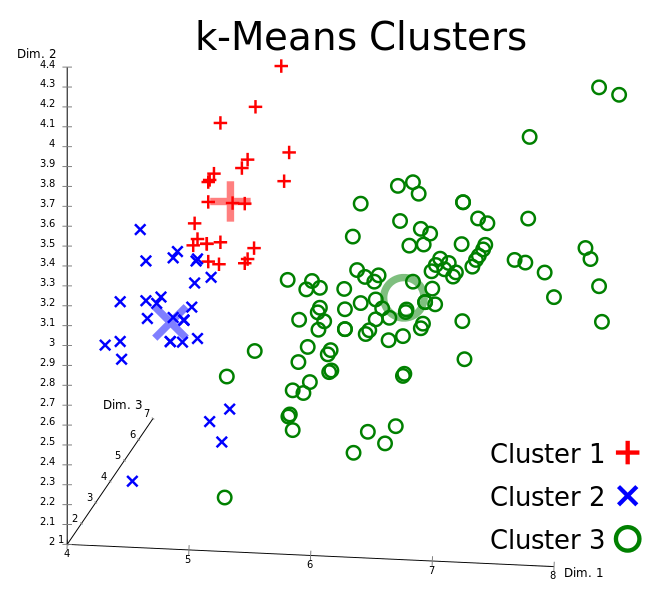
\includegraphics[width=0.6\textwidth]{MarcoTeorico/Imagenes/imagencluster.png}
            \caption{Ejemplo de agrupamiento.}                       
            \label{fig:Cap2_3_2_1}
    \end{figure} 
    
\hspace*{1cm}Los métodos de agrupamiento se pueden dividir en paramétricos y no paramétricos. Entre los métodos de agrupamiento paramétricos se encuentran las mixturas finitas, éstas son una poderosa herramienta para modelar densidades de probabilidad de conjuntos de datos univariados y multivariados, modelan observaciones las cuales se asume que han sido producidas por un conjunto de fuentes aleatorias alternativas e infieren los parámetros de estas fuentes para identificar qué fuente produjo cada observación, lo que lleva a un agrupamiento del conjunto de observaciones. Los métodos de agrupamiento no paramétricos pueden dividirse en tres grupos fundamentales: jerárquicos, particionales y basados en densidad.

 \subsubsection {Algoritmos jerárquicos}
Según \cite{[PASPLASA]} los algoritmos jerárquicos son aquellos en los que se va particionando el conjunto de datos por niveles, de modo que en cada nivel generalmente se unen o dividen dos grupos del nivel anterior de acuerdo al tipo de algoritmo: aglomerativo o divisivo. Según \cite{[DUHASTO]} las estrategias jerárquicas más conocidas son:
 \begin{itemize}
 \item \textbf{Single Link (SL): }En cada paso se unen los dos grupos cuyos elementos más cercanos 
tienen la mínima distancia.
 \item \textbf{Average Link (AL): }En cada paso se unen los dos grupos que tienen la mínima distancia promedio entre sus puntos.
 \item \textbf{Complete Link (CL): }En cada paso se unen los dos grupos tal que su unión tiene el diámetro mínimo o los dos grupos con la menor distancia máxima entre sus elementos.  
\item \textbf{Chameleon (AC): } Según \cite{[KARHANKU]} este método consta de dos fases. En la primera fase se construye un grafo con los  $k$ vécinos más cercanos y usa un algoritmo de partición para agrupar los puntos en subgrupos. En la segunda fase usa un algoritmo jerárquico aglomerativo para encontrar los clusters genuinos combinando repetidamente estos subgrupos. Esta fase determina el par de subgrupos más similares tomando en cuenta su conectividad y cercanía. A diferencia del algoritmo SL, este algoritmo permite unir varios pares de subgrupos en la misma iteración.
\end{itemize}
 
\subsubsection {Algoritmos particionales}
Los algoritmos particionales son los que realizan una división inicial de los datos en grupos y luego mueven los objetos de un grupo a otro según se optimice alguna función objetivo. Algunos de estos son:
 
\begin{itemize} 
 \item \textbf{Algoritmo K-Means: } Según \cite{[DUHASTO]}, la idea principal de este algoritmo es definir k centroides (uno para cada grupo) y luego tomar cada punto y situarlo en la clase de su centroide más cercano. El próximo paso es recalcular el centroide de cada grupo y volver a distribuir todos los puntos según el centroide más cercano. El proceso se repite hasta que ya no hay cambio en los grupos dentro del proceso iterativo.
 \item \textbf{Algoritmo CURE: }De acuerdo a \cite{[GURASHI]} este algoritmo es un enfoque híbrido entre los dos enfoques (jerárquico y particional), que trata de emplear las ventajas de ambos y de eliminar las limitaciones. En lugar de usar un solo punto como representante de un grupo se emplea $n$ puntos representativos del grupo. La similaridad entre dos grupos se mide por la similaridad del par de puntos representativos más cercanos, uno de cada grupo.
Para tomar los puntos representativos selecciona los $n$ puntos más dispersos y los atrae hacia el centro del mismo por un factor de contracción ${\alpha }$; en cada paso se unen los dos grupos más cercanos y una vez unidos se vuelve a calcular para éste su centro y los c puntos representativos.
\end{itemize}
 
\subsubsection {Algoritmos basados en densidad}
Los algoritmos basados en densidad enfocan el problema de la división de una base de datos en grupos teniendo en cuenta la distribución de densidad de los puntos, de modo tal que los grupos que se forman tienen una alta densidad de puntos en su interior mientras que entre ellos aparecen zonas de baja densidad. Entre los algoritmos que emplean esta técnica se pueden mencionar:
 
\begin{itemize} 
\item \textbf{Algoritmo DBSCAN:} Como se indica en \cite{[ESKRISAXU]} el algoritmo comienza seleccionando un punto p arbitrario y si p es un punto central, se comienza a construir un grupo y se ubican en su grupo todos los objetos denso-alcanzables desde p. Si p no es un punto central se visita otro objeto del conjunto de datos.\\
El proceso continúa hasta que todos los objetos han sido procesados. Los puntos que quedan fuera de los grupos formados se llaman puntos ruido y los puntos que no son ni ruido ni centrales se llaman puntos borde.\\
De esta forma DBSCAN construye grupos en los que sus puntos son o puntos centrales o puntos borde, un grupo puede tener más de un punto central. 
\item \textbf{Algoritmo OPTICS:} Según \cite{[ANBRUKRISA]} la motivación para la realización de este algoritmo se basa en la necesidad de introducir parámetros de entrada en casi todos los algoritmos de agrupamiento existentes que en la mayoría de los casos son difíciles de determinar, además en conjuntos de datos reales no existe una manera de determinar estos parámetros globales, el algoritmo OPTICS trata de resolver este problema basándose en el esquema del algoritmo DBSCAN creando un ordenamiento de la base de datos para representar la estructura del agrupamiento basada en densidad, además puede hacer una representación gráfica del agrupamiento incluso para conjuntos de datos grandes.
\end{itemize}